\documentclass[UTF8,fontset=windows,12pt]{ctexart}
%\setcounter{tocdepth}{1}
%\setcounter{secnumdepth}{4}
%\usepackage{ctex} %若要输入中文请取消注释或者把article改成ctexart
% This first part of the file is called the PREAMBLE. It includes
% customizations and command definitions. The preamble is everything
% between \documentclass and \begin{document}.
%\usepackage[OT1]{fontenc}
%\usepackage{fontspec}
%\setmainfont{Times New Roman}
%\setCJKmainfont{Microsoft YaHei}
\usepackage[left=1.91cm,right=1.91cm,top=2.54cm,bottom=2.54cm]{geometry}
\usepackage{amsfonts}
\usepackage{amsmath}
\usepackage{amssymb}
\usepackage[upint,lcgreekalpha]{stix}
\usepackage[type1]{garamondlibre}
%\usepackage{esint}
\usepackage{pgfplots}
\pgfplotsset{compat=1.18}
\usepackage{tikz}
\usetikzlibrary{arrows}
\usepackage{extarrows}
\usepackage[only,llbracket,rrbracket]{stmaryrd}
\usepackage{titlesec}
\usepackage{bm}
\usepackage{graphicx}
\usepackage{appendix}
\usepackage{tikz-cd}
\usepackage{tikz-3dplot}
\usetikzlibrary{arrows.meta, decorations.pathreplacing, calc, patterns}
\usepackage{float}
\usepackage{mathtools}
\usepackage{amsthm}
\usepackage{verbatim}              % better theorem environments
\usepackage{setspace}
\usepackage{enumitem}
\setenumerate[1]{itemsep=0pt,partopsep=0pt,parsep=\parskip,topsep=5pt}
\setitemize[1]{itemsep=0pt,partopsep=0pt,parsep=\parskip,topsep=5pt}
\setdescription{itemsep=0pt,partopsep=0pt,parsep=\parskip,topsep=5pt}
\usepackage{xcolor}
\usepackage[colorlinks,linkcolor=black,anchorcolor=black,citecolor=black]{hyperref}
%\usepackage{apacite}
\usepackage[numbers]{natbib}
%\usepackage{showkeys}
\usepackage{cases}
\usepackage{fancyhdr}
\usepackage[scaled=0.92]{helvet}	% set Helvetica as the sans-serif font
%\usepackage{upgreek}
%\renewcommand{\rmdefault}{ptm}		% set Times as the default text font
%\usepackage{newtxtext}
\bibliographystyle{plain}
% If AMS-LaTeX is used, it can be loaded before or after mtpro2		
% The following loads metro and defines some common MTPro options [2, 4]
%\usepackage[lite,subscriptcorrection,nofontinfo]{mtpro2}
%\pdfmapfile{+mtpro2.map}

%\usepackage{txfonts}

% various theorems, numbered by section

\makeatletter
\renewenvironment{proof}[1][\proofname]{\par
  \pushQED{\qed}%
  \normalfont \topsep6\p@\@plus6\p@\relax
  \trivlist
  \item[\hskip\labelsep
        \bfseries % 关键修改:斜体改为加粗
        #1\@addpunct{.}]\ignorespaces
}{%
  \popQED\endtrivlist\@endpefalse
}
\makeatother
\newtheoremstyle{kaiti-theorem}   % 样式名称
  {3pt}                           % 上方间距
  {3pt}                           % 下方间距
  {\kaishu\upshape}               % 正文字体:中文楷体 + 英文直立
  {}                              % 缩进量
  {\bfseries\upshape}      % 头部字体(定理名):中文楷体粗体 + 英文直立粗体
  {.}                             % 定理名后标点
  {0.5em}                         % 定理名后间距
  {}                              % 头部说明(留空)

% 应用自定义样式
\theoremstyle{kaiti-theorem}
\newtheorem{thm}{定理}[section]
\newtheorem{nota}[thm]{记号}
\newtheorem{question}{问题}
\newtheorem*{questionn}{思考}
\newtheorem{exe}{习题}[section]
\newtheorem{assump}[thm]{假设}
\newtheorem*{thmm}{定理}
\newtheorem{defn}{定义}[section]
\newtheorem{lem}[thm]{引理}
\newtheorem*{lemm}{引理}
\newtheorem{prop}[thm]{命题}
\newtheorem*{propp}{命题}
\newtheorem*{claim}{断言}
\newtheorem{cor}[thm]{推论}
\newtheorem{conj}[thm]{猜想}
\newtheorem{rmk}{注记}[section]
\newtheorem{ex}{例}[section]
\newtheorem{pf}{证明}
\newtheorem{problem}{作业题}
\numberwithin{equation}{section}





\DeclareMathOperator{\id}{id}
\DeclareMathOperator*{\esssup}{ess\,sup}
\renewcommand{\Re}{\textbf{Re}\,}  
\renewcommand{\Im}{\textbf{Im}\,}  
\newcommand{\R}{\mathbb{R}}  
\newcommand{\FH}{\mathbb{H}}  
\newcommand{\C}{\mathbb{C}}  
\newcommand{\Z}{\mathbb{Z}}
\newcommand{\X}{\mathbb{X}}
\newcommand{\N}{\mathbb{N}}
\newcommand{\Q}{\mathbb{Q}}
\newcommand{\T}{\mathbb{T}}
\newcommand{\TT}{\mathcal{T}}
\newcommand{\TP}{\overline{\partial}{}}
\newcommand{\TJ}{\langle\TP\rangle}
\newcommand{\TL}{\overline{\Delta}{}}
\newcommand{\curl}{\text{curl }}
\newcommand{\dive}{\text{div }}
\newcommand{\bd}[1]{\mathbf{#1}}  % for bolding symbols
\newcommand{\bds}[1]{\boldsymbol{#1}}  % for bolding symbols
\newcommand{\RR}{\mathcal{R}}      % for Real numbers
\newcommand{\sh}{\mathcal{S}}  
\newcommand{\sph}{\mathbb{S}}  
\newcommand{\Om}{\Omega}
\newcommand{\OmT}{{\Omega_T}}
\newcommand{\ut}{{U_T}}
\newcommand{\vp}{\varphi}
\newcommand{\Th}{\Theta}
\newcommand{\Lam}{\Lambda}
\newcommand{\Omb}{{\overline{\Omega}}}
\newcommand{\OmbT}{{\overline{\Omega_T}}}
\newcommand{\ub}{{\overline{U}}}
\newcommand{\ubt}{{\overline{U_T}}}
\newcommand{\q}{\quad}
\newcommand{\p}{\partial}
\newcommand{\pb}{\boldsymbol{\partial}}
\newcommand{\lap}{\Delta}
\newcommand{\dd}{\mathfrak{D}}
\newcommand{\DD}{\mathcal{D}}
\newcommand{\den}{{\bar\rho}_{0}}
\newcommand{\Dt}{{\p}_{t}+v^{k}{\p}_{k}}
\newcommand{\col}[1]{\left[\begin{matrix} #1 \end{matrix} \right]}
\newcommand{\noi}{\noindent}
\newcommand{\nab}{\nabla}
\newcommand{\cnab}{\overline{\nab}}
\newcommand{\cp}{\overline{\partial}{}}
\newcommand{\dx}{\,\mathrm{d}x}
\newcommand{\dxx}{\,\mathrm{d}\bds{x}}
\newcommand{\xxi}{\boldsymbol{\xi}}
\newcommand{\eeta}{\boldsymbol{\eta}}
\newcommand{\dxxi}{\,\mathrm{d}\boldsymbol{\xi}}
\newcommand{\deeta}{\,\mathrm{d}\boldsymbol{\eta}}
\newcommand{\dxi}{\,\mathrm{d}\xi}
\newcommand{\deta}{\,\mathrm{d}\eta}
\newcommand{\dy}{\,\mathrm{d}y}
\newcommand{\dyy}{\,\mathrm{d}\bds{y}}
\newcommand{\dz}{\,\mathrm{d}z}
\newcommand{\dzz}{\,\mathrm{d}\bds{z}}
\newcommand{\dph}{\,\mathrm{d}\varphi}
\newcommand{\dt}{\,\mathrm{d}t}
\newcommand{\dr}{\,\mathrm{d}r}
\newcommand{\dtt}{\,\mathrm{d}\tau}
\newcommand{\dS}{\,\mathrm{d}S}
\newcommand{\dss}{\,\mathrm{d}\sigma}
\newcommand{\dmu}{\,\mathrm{d}\mu}
\newcommand{\dnu}{\,\mathrm{d}\nu}
\newcommand{\dV}{\,\mathrm{d}V}
\newcommand{\ds}{\,\mathrm{d}s}
\newcommand{\drr}{\,\mathrm{d}\rho}
\newcommand{\dist}{\text{dist }}
\newcommand{\vol}{\text{vol}\,}
\newcommand{\volo}{\text{vol}(\Omega)}
\newcommand{\spt}{\text{Spt}\,}
\newcommand{\Tr}{\text{Tr}\,}
\newcommand{\lee}{\langle}
\newcommand{\ree}{\rangle}
\newcommand{\xee}{\langle\xi\rangle}
\newcommand{\xxee}{\langle\boldsymbol{\xi}\rangle}
\newcommand{\xeta}{\langle\eta\rangle}
\newcommand{\xeeta}{\langle\boldsymbol{\eta}\rangle}
\newcommand{\kk}{\kappa}
\newcommand{\lam}{\lambda}
\newcommand{\io}{\int_{\Omega}}
\newcommand{\iu}{\int_{U}}
\newcommand{\is}{\int_{\Sigma}}
\newcommand{\ipo}{\int_{\partial\Omega}}
\newcommand{\ipu}{\int_{\partial U}}
\newcommand{\ig}{\int_{\Gamma}}
\newcommand{\ir}{\int_{\R}}
\newcommand{\ird}{\int_{\R^d}}
\newcommand{\irn}{\int_{\R^n}}
\newcommand{\fpi}{\frac{1}{(2\pi)^{\frac{d}{2}}}}
\newcommand{\ddt}{\frac{\mathrm{d}}{\mathrm{d}t}}
\newcommand{\ddx}{\frac{\mathrm{d}}{\mathrm{d}x}}
\newcommand{\eps}{\varepsilon}
\providecommand{\jump}[1]{\left\llbracket #1 \right\rrbracket }
\providecommand{\len}[1]{\lee #1 \ree }
\providecommand{\ino}[1]{\left\| #1 \right\| }
\providecommand{\bno}[1]{\left| #1 \right| }
\newcommand{\red}{\textcolor{red}}
\newcommand{\green}{\textcolor{green}}
\newcommand{\blue}{\textcolor{blue}}
\newcommand{\nnr}{{[n+1]}}
\newcommand{\nnn}{{[n]}}
\newcommand{\nnl}{{[n-1]}}
\newcommand{\nnll}{{[n-2]}}	
\newcommand{\mmr}{{[m+1]}}
\newcommand{\mmm}{{[m]}}
\newcommand{\mml}{{[m-1]}}
\newcommand{\mmll}{{[m-2]}}

%---------------Special variables--------------
\newcommand{\CC}{\mathfrak{C}}  
\newcommand{\NN}{\mathbf{N}}
\newcommand{\LH}{\mathcal{L}}
\newcommand{\HH}{\mathcal{H}}  
\newcommand{\EE}{\mathcal{E}}  
\newcommand{\FT}{\mathcal{F}}  
\newcommand{\fT}{\mathbf{T}}  
\newcommand{\FA}{\mathbf{A}}  
\newcommand{\MH}{\mathcal{M}}
\newcommand{\NH}{\mathcal{N}}
\newcommand{\PH}{\mathcal{P}}
\newcommand{\VH}{\mathcal{V}}
\newcommand{\XX}{\mathfrak{X}}
\newcommand{\xx}{{\bds{x}}}
\newcommand{\bx}{\mathbf{x}}
\newcommand{\by}{\mathbf{y}}
\newcommand{\bp}{\mathbf{p}}
\newcommand{\bq}{\mathbf{q}}
\newcommand{\pp}{{\bds{p}}}
\newcommand{\qq}{{\bds{q}}}
\newcommand{\uu}{\mathbf{u}}
\newcommand{\ww}{\mathbf{w}}
\newcommand{\vv}{\mathbf{v}}
\newcommand{\yy}{{\bds{y}}}
\newcommand{\zz}{{\bds{z}}}
\newcommand{\zo}{\mathbf{0}}
\newcommand{\ee}{\mathbf{e}}
\newcommand{\fa}{\mathbf{a}}
\newcommand{\fb}{\mathbf{b}}
\newcommand{\fc}{\mathbf{c}}
\newcommand{\ff}{\bds{f}}
\newcommand{\fr}{\mathbf{r}}
\newcommand{\fh}{\mathbf{h}}
\newcommand{\fm}{\mathbf{m}}
\newcommand{\fg}{\mathbf{g}}
\newcommand{\FF}{\mathbf{F}}
\newcommand{\GG}{\mathbf{G}}
\newcommand{\BB}{\mathbf{B}}



\begin{document}
\title{\LARGE{\bf  2025年秋季学期偏微分方程作业一}}
\date{截止时间:2025年11月27日下课前}

\maketitle

\begin{problem}[习题1.1.2]
解方程$x\p_t u+t\p_x u=0~(t,x\in\R),~u(0,x)=e^{-x^2}$. 并说明$tOx$平面中哪些部分的解由初值唯一确定?
\end{problem}

\begin{problem}[习题1.1.3]
考虑方程$3u_y+u_{xy}=0$.
\begin{itemize}
\item [(1)] 计算方程的通解. (提示: 令$v=\p_y u$.)
\item [(2)] 若假设$u(x,0)=e^{-3x},~u_y(x,0)=0$, 方程的解是否存在?是否唯一?
\end{itemize}
\end{problem}



\begin{problem}[习题2.1.1]
证明方程$u_{tt}-c^2u_{xx}=0$的解必定满足“平行四边形法则”,即$u(A)+u(C)=u(B)+u(D)$, 其中 $A,B,C,D$ 构成 $xOt$-平面 上的平行四边形,其边界方程为$x\pm ct=\text{常数}$. 

\begin{figure}[H]
\centering
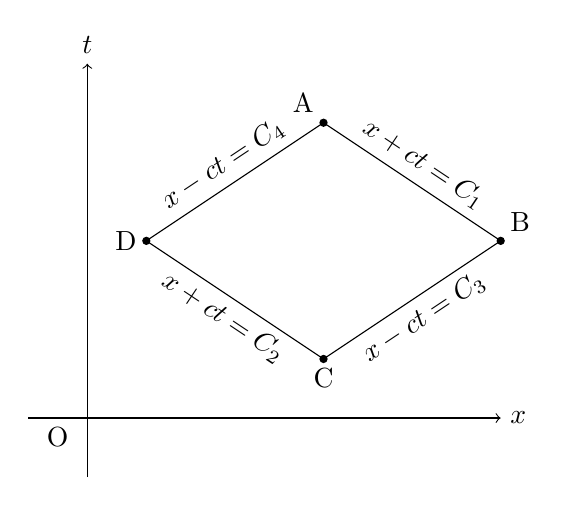
\begin{tikzpicture}[scale=0.75]
% 坐标轴
\draw[->] (-1,0) -- (7,0) node[right] {$x$};
\draw[->] (0,-1) -- (0,6) node[above] {$t$};

% 定义顶点坐标
\coordinate (A) at (4,5);
\coordinate (B) at (7,3);
\coordinate (C) at (4,1);
\coordinate (D) at (1,3);
\coordinate (O) at (-0.5,0);
% 绘制平行四边形边并标注直线方程
\draw (A) -- (B) node[pos=0.5, above, sloped] {$x+ct=C_1$};
\draw (B) -- (C) node[pos=0.5, below, sloped] {$x-ct=C_3$};
\draw (C) -- (D) node[pos=0.5, below, sloped] {$x+ct=C_2$};
\draw (D) -- (A) node[pos=0.5, above, sloped] {$x-ct=C_4$};

% 标记顶点
\node[above left] at (A) {A};
\node[above right] at (B) {B};
\node[below] at (C) {C};
\node[left] at (D) {D};
\node[below] at (O) {O};

% 绘制顶点实心圆点
\foreach \point in {A,B,C,D}
    \fill (\point) circle (2pt);
\end{tikzpicture}
\caption{习题2.1.1图}
\end{figure}
\end{problem}

\begin{problem}[习题2.1.2]
考虑方程 $20u_{tt}-u_{tx}-u_{xx}=0~(t>0,x\in\R)$.
\begin{itemize}
\item  [(1)] 计算通解。(提示:因式分解方程左边的微分算子)
\item  [(2)] 假设初值是 $u(0,x)=x,~\p_t u(0,x)=e^{-x}+\frac14$, 计算方程的解$u(t,x)$.
\end{itemize}
\end{problem}

\begin{problem}[习题2.1.3]
考虑第一象限中一个扇形区域内的波动方程
\begin{equation*}
\begin{cases}
u_{tt}-u_{xx}=0&~~t>x>0;\\
u(t,t)=\vp(t),~u_x(t,0)=\psi(t)&~~t\geq 0.
\end{cases}
\end{equation*}
\begin{itemize}
\item [(1)] 通过将初值$\vp,\psi$代入通解$u(t,x)=F(x-t)+G(x+t)$, 计算$u(t,x)$ (用$\vp,\psi$表示).
\item [(2)] 对哪些$(t,x)$, $u(t,x)$的值完全由初值$\vp,\psi$在$[0,1]$区间内的部分决定? 
\end{itemize}
\end{problem}

\begin{problem}[习题2.1.4]
考虑一维波方程的初值问题
\begin{equation*}
\begin{cases}
u_{tt}-c^2u_{xx}=0&~~t>0,~x\in\R\\
u(0,x)=\varphi(x),~u_t(0,x)=\psi(x)&~~t=0,~x\in\R,\\
\end{cases}
\end{equation*}其中 $c>0$ 是给定的常数, $\varphi,\psi\in C_c^{\infty}(\R)$. 定义$$K(t):=\frac12\int_\R |\p_t u(t,x)|^2\dx,~P(t):=\frac{c^2}{2}\int_\R|\p_x u (t,x)|^2\dx.$$ 证明:
\begin{itemize}
\item [(1)]  $K(t)+P(t)$是守恒量,并据此证明方程平方可积解的唯一性。
\item [(2)]  当$t$充分大时,有$K(t)=P(t)$. (提示:使用达朗贝尔公式)
\end{itemize}
本题中的记号$C_c^\infty(\R)$是指全体具有紧支集的光滑函数,即$C_c^\infty(\R):=\{f\in C^\infty(\R):\spt f\text{是紧集}\}$, 其中$\spt f:=\overline{\{f(\xx)\neq 0\}}$.
\end{problem}

\begin{problem}[习题2.2.3]
设复值函数$u(t,\xx)=e^{i(\yy\cdot\xx-\sigma t)}$, 其中$\sigma\in\C,~\xx,\yy\in\R^d$. 对如下方程具有该形式的解,计算$\sigma$与$|\yy|$之间的关系(该关系称作“色散关系”)。
\begin{itemize}
\item [(1)] 波动方程 $\p_t^2 u-\lap u=0$.
\item [(2)] Klein-Gordon方程 $\p_t^2 u-\lap u+m^2u=0$, 这里$m>0$是常数.
\item [(3)] Schr\"odinger方程 $i\p_t u+\lap u=0$.
\item [(4)] Airy方程 $\p_t u+\p_x^3 u=0$, 本例中$d=1$.
\end{itemize}
\end{problem}


\begin{problem}[习题2.3.3]
证明:对\underline{任意常数}$D\in\R$, 如下方程至多只有一个光滑解 $u\in C^{\infty}([0,T]\times[0,1])$.
\begin{equation}
\begin{cases}
\p_t^2 u+D\p_t u-\p_x^2 u=0~~~&t\in(0,T), x\in(0,1);\\
u(0,x)=\varphi(x),~\p_t u(0,x)=\psi(x)~~~&x\in [0,1];\\
u(t,0)=u(t,1)=0~~~&t\in[0,T].
\end{cases}
\end{equation}
\end{problem}


\begin{problem}[问题2.2.1,选做]
考虑二维波动方程的初值问题
\[
\p_t^2 u-\lap u=0~~(t>0,\xx\in\R^2),\q\q u(0,\xx)=0,~~\p_tu(0,\xx)=\psi(\xx)~~(\xx\in\R^d).
\]其中初值$\psi\in C_c^\infty(\R^2)$.
\begin{itemize}
\item [(1)] 用积分的极坐标表示证明 $$u(t,\xx)=\frac{1}{2\pi}\int_0^t \frac{r}{\sqrt{t^2-r^2}}\int_{\p B(\bd{0},1)}\psi(\xx+r\zz)\dS_\zz\dr.$$
\item [(2)] 证明: 存在常数$C>0$(不依赖$\psi$),使得如下估计成立 $$|u(t,\xx)|\leq \frac{C}{\sqrt{t}}\left(\int_{\R^2}|\psi(\yy)|\dyy+\int_{\R^2}|\nab\psi(\yy)|\dyy\right).$$
\end{itemize}

(2)的提示:把(1)右边的积分$\int_0^t$拆成$\int_0^{t-\eps}+\int_{t-\eps}^t$. 第二部分的估计和三维情况类似。对第一部分,把$r\leq t-\eps$带进(1)中的分母,然后取$\eps>0$充分小去得到要证的结果。
\end{problem}

\end{document}
